\documentclass[../pheader.tex]{subfiles}

\begin{document}
{\sc Ayudantía 1 - EDO\hfill \small\rm Apuntes: Sebastián Sánchez}

\begin{center}
    \begin{tabular}{rl}
        Docente:& Nikola Kamburov\\
        Ayudante:& Jorge Acuña
    \end{tabular}
\end{center}

% PROBLEMA 1
\begin{problema}
Resuelva y encuentre el intervalo máximal del problema:
\[
    t\dot{y} + 2y = 4t^2
    ,\quad
    y(1) = a
    \qquad a\in \mathbb{R}.
\]
\end{problema}
\begin{proof}
Dado que el PVI está en \(t_0 = 1\), los tiempos que consideramos están lejos de
cero, así podemos dividir por \(t\). Despejando obtenemos la siguiente
ecuación
\[
    \dot{y} = 4t - \frac{2}{t} y.
\]
Usando el método del factor integrante/propagador se tiene que
\[
    P(t,s)
    =
    \exp\left(\int_{s}^{t} -\frac{2 du}{u}\right)
    =
    \exp\left(\log(s^2) - \log(t^2)\right)
    =
    s^{2} t^{-2}
.\]
Así, la solución \(\phi(t)\) está definida como
\begin{align*}
    \phi(t)
    &= y(1) P(t,1) + \int_{1}^{t} P(t,s) 4s ds
    \\&= a t^{-2} + t^{-2} \int_{1}^{t} 4 s^3 ds
    \\&= a t^{-2} + (t^{2} - t^{-2})
    \\&= t^{2} + t^{-2} (a - 1).
\end{align*}
Deducimos que si \(a = 1\), entonces la solución es válida para todo tiempo
\(t\). Por otro lado, si \(a \ne 1\) entonces \(t\ne 0\) y como estamos
trabajando de \(t = 1\) concluimos que el intervalo máximo es
\(t\in (0, \infty)\).
\end{proof}

% PROBLEMA 2
\begin{problema}
Definamos
\[
    f(y) \coloneqq
    \begin{cases}
        y^3 \sin (y^{-1}) &, y\in \mathbb{R}\setminus \left\{0\right\}\\
        0 &, y = 0.
    \end{cases}
\]
Para \(y_0\in \mathbb{R}\), considere el problema
\(
    \quad \dot{y} = f(y),\quad y(0) = y_0
\).\\
Analize los casos en que (1) \(\abs{y_0} > 1/\pi\) y (2) \(\abs{y_0} \le
1/\pi\) y encuentre los intervalos máximos de la solución en cada caso. En particular,
para el caso (2) demuestre que el intervalo máximal de la solución es todo
\(\mathbb{R}\), siendo la solución \(y(t;y_0)\) monótona y acotada. Encuentre el límite
\(
    \lim_{t\to \pm \infty} y(t;y_0)
.\)
\end{problema}
\begin{proof} \ \\
\begin{plist}
\item Partamos con el caso \(\abs{y_0} > 1/\pi\). Dado que hay un valor
absoluto, debemos analizar dos subcasos.
\begin{clist}
    \item Para \(y_0 > 1/\pi\), estamos trabajando lejos de \(0\) así que la
    ecuación que usamos es
    \[
        \dot{y} = y^3 \sin (y^{-1}).
    \]
    Y por la misma razón podemos pasar dividiendo, dejándonos que la inversa de
    la solución es
    \[
        \int_{y_0}^{y} \frac{du}{u^3 \sin(u^{-1})} = F(t;y_0).
    \]
    Aquí podríamos intentar resolver la ecuación, sin embargo, dado que nos
    piden el intervalo máximo de definición de la solución podemos ahorrarnos
    ese trabajo.

    Recordando que el dominio de una función es el recorrido de su inversa, para
    encontrar en qué tiempos es válida la solución basta con ver el recorrido de
    \(F(t;y_0)\).

    Notar que en \(F(t;y_0)\), \(y\) se mueve entre \(\left(1/\pi,
    \infty\right)\), entonces tanto \(u^3\) como \(\sin(u^{-1})\) son positivas
    (usando la convención de \(1/\infty = 0\)). Se sigue que \(F(t;y_0)\) es
    creciente.

    Dado que \(F(t;y_0)\) es creciente y continua, su máximo y mínimo los
    alcanza en los extremos. Luego
    \[
        T_{+} = \underset{y \uparrow \infty}{\lim} F(t;y_0) = a_{+}
        \hspace{1cm}
        T_{-} = \underset{y \downarrow \frac{1}{\pi}}{\lim} F(t;y_0) = -\infty
    .\]
    Donde \(a_{+}\in \mathbb{R}^{+}\) pues la integral es convergente (está acotada
    por \(\int \frac{1}{u^2}\)).

    \item Para \(y_0 < -1/\pi\), trabajamos con la misma ecuación. De esta forma
    tenemos que la inversa de la solución es
    \[
        \int_{y_0}^{y} \frac{du}{u^3 \sin(u^{-1})} = F(t;y_0)
    .\]
    Donde \(y\) ahora se mueve desde \((-\infty,-1/\pi)\)
    y por consiguiente tanto \(u^{3}\) como \(\sin(u^{-1})\) son negativas. Se
    concluye entonces que \(F(t;y_0)\) es creciente. Luego, los tiempos máximos
    y mínimos para los cuales está definida la solución son
    \begin{center}
    \begin{tabular}{L L L}
        T_{-} &= \underset{y \to -\infty^{+}}{\lim} F(t;y_0) &= a_{-}\\
        T_{+} &= \underset{y \to (-\frac{1}{\pi})^{-}}{\lim} F(t;y_0) &= \infty
    \end{tabular}
    \end{center}
    Donde \(a_{-}\in \mathbb{R}^{-}\) por la misma cota de arriba.
\end{clist}

\item Para el caso \(\abs{y_0} < 1/\pi\), notemos que \(f(y)\) se anula para \(y=0\) y
\(y = 1/k\pi\) (\(k\in \mathbb{Z}\setminus \left\{0\right\}\). Luego, tenemos que
analizar cada uno de estos casos. Estos se reducen a ver
\(y_0 \in \left(\frac{1}{(k+1)\pi}, \frac{1}{k\pi}\right)\) y \(y_0 = 0\).
\begin{clist}
    \item Si \(y_0 = 0\), entonces \(\dot{y}(0) = 0\) y concluimos que la
    solución es la función constante \(0\).

    \item Si \(k\) es positivo y \(\frac{1}{(k+1)\pi} < y_0 < \frac{1}{k\pi}\),
    como estamos lejos de \(0\) podemos obtener la inversa de la solución
    despejando la ecuación inicial, esto nos deja con
    \[
        F(y;y_0) = \int_{y_0}^{y} \frac{du}{u^3 \sin (u^{-1})}
    .\]
    Donde \(y\in \left(1/(k+1)\pi, 1/k\pi\right)\). Para determinar
    si \(F(y;y_0)\) es creciente o no es necesario saber la paridad de \(k\).

    Para \(k\) par, el seno es positivo y por lo tanto \(F(y;y_0)\) es
    creciente. Luego, el intervalo máximo de la solución está dado por
    \[
        T_{+} = \underset{y \uparrow \frac{1}{k\pi}}{\lim} F(t;y_0) = \infty
        \hspace{1cm}
        T_{-} = \underset{y \downarrow \frac{1}{(k+1)\pi}}{\lim} F(t;y_0) = -\infty
    .\]
    Con esta información podemos deducir que la solución \(y(t;y_0)\) es
    creciente, pues
    \[
        \lim_{t\to \infty} y(t;y_0) = \frac{1}{k\pi}
        >
        \frac{1}{(k+1)\pi} = \lim_{t\to -\infty} y(t;y_0)
    .\]

    Por otro lado, si \(k\) es impar, el seno es negativo y por lo tanto la
    función \(F(y;y_0)\) es decreciente. De esta forma el intervalo máximo es
    \[
        T_{+} = \underset{y \uparrow \frac{1}{k\pi}}{\lim} F(t;y_0) = -\infty
        \hspace{1cm}
        T_{-} = \underset{y \downarrow \frac{1}{(k+1)\pi}}{\lim} F(t;y_0) = \infty
    .\]
    Y concluimos que la solución es decreciente, pues
    \[
        \lim_{t\to \infty} y(t;y_0) = \frac{1}{(k+1)\pi}
        <
        \frac{1}{k\pi} = \lim_{t\to -\infty} y(t;y_0)
    .\]

    \item Para \(k\) negativo, el análisis es similar.
\end{clist}
\end{plist}
\end{proof}

% PROBLEMA 3
\begin{problema}
Considere el PVI
\[
    \dot{y} = 3t^2 \abs{y}^{2/3}
    \hspace{1cm}
    y(0) = 0
.\]
Y construya una familia infinita de soluciones.
\end{problema}
\begin{proof}
En primer lugar notemos \(y\equiv 0\) es una solución trivial.

Analicemos el caso \(y > 0\). Despejando e integrando obtenemos la solución
general
\[
    y(t) =  \frac{1}{27} t^9
.\]
Luego, para cada \(n \in \mathbb{N}\) la familia infinita de funciones
\[
    y_n (t) =
    \begin{cases}
        (t - n)^9/27 & t \ge n \\
        0 & t < n
    \end{cases}
.\]
cumple con lo pedido.
\end{proof}

% PROBLEMA 4
\begin{problema}
Haga un análisis cualitativo de la ecuación
\[
    \dot{x} = x^2 - \frac{t^2}{1+t^2}
.\]
\begin{plist}
    \item Demuestre que existe una única solución que se aproxima
    asintóticamente a la recta \(x=1\).

    \item Demuestre que todas las soluciones bajo esta solución se aproximan
    asintóticamente a la recta \(x=-1\).

    \item Demuestre que todas las soluciones sobre esta solución tienden a
    \(+\infty\) en tiempo finito.
\end{plist}
\end{problema}
\begin{proof} \ \\
\begin{plist}
    \item Notemos que \(u(t) \equiv 1\) es una subsolución. Por otro lado,
    reescribiendo la ecuación como
    \[
        \dot{x} =
        \left(x - \frac{t}{\sqrt{1 + t^2}}\right)
        \left(x + \frac{t}{\sqrt{1 + t^2}}\right)
    .\]
    Vemos que \(l(t) = t/\sqrt{1 + t^2}\) es una supersolución (es una
    0-isoclina).
    \begin{center}
    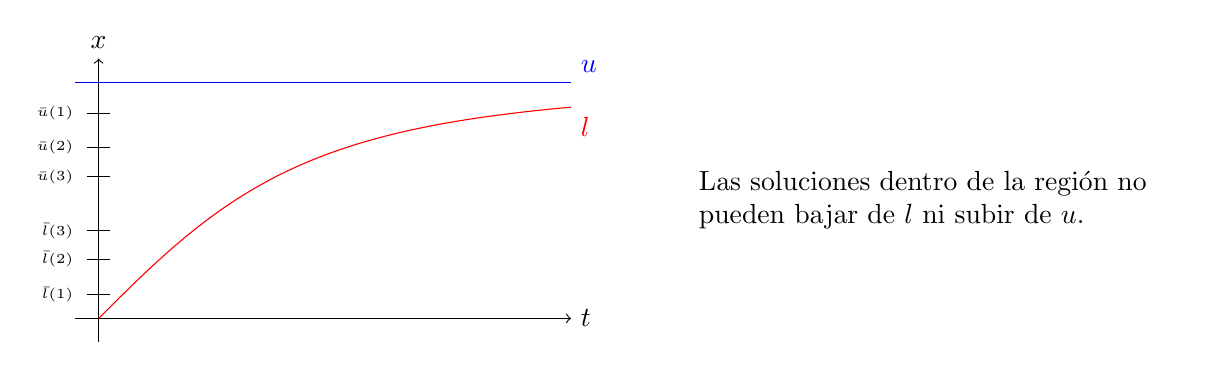
\begin{tikzpicture}[scale=3]
        % Region atrapada
        \def\x{2};
        \draw[->] (-.1, 0) -- (\x, 0) node[right] {\(t\)};
        \draw[->] (0, -.1) -- (0, 1.1) node[above] {\(x\)};
        \draw[blue] (-0.1,1) -- (\x,1) node[above right] {\(u\)};
        \draw[domain=0:\x, smooth, variable=\t, red]
            plot ({\t}, {\t/sqrt(1+\t*\t)}) node[below right] {\(l\)};
        % Puntos iniciales de soluciones
        \foreach \u/\label in {1.3/1,1.6/2,2/3}
        \draw (-.05,{1/\u + .1}) -- (.05, {1/\u + .1})
            node[left = 10pt] {\tiny \(\bar{u}(\label)\)};
        \foreach \l/\label in {2.7/3,4/2,10/1}
        \draw (-.05,{1/\l}) -- (.05, {1/\l})
            node[left = 10pt] {\tiny \(\bar{l}(\label)\)};
        % Texto
        \begin{scope}[xshift=2.5cm,yshift=.5cm]
        \node[right, text width=6cm]
        {%
        Las soluciones dentro de la región no
        pueden bajar de \(l\) ni subir de \(u\).
        };
        \end{scope}
    \end{tikzpicture}
    \end{center}
    Para cada tiempo \(t\), a la solución que pasa por \(u(t)\) o \(l(t)\),
    vamos a denotar por \(\bar{u}(t)\) y \(\bar{l}(t)\) al corte de esa
    solución con el eje \(x\).
    Luego, \(\left(\bar{u}(t)\right)_{t\in \mathbb{N}}\) es una sucesión
    estrictamente decreciente (dado que las soluciones no se cruzan) y por ser
    acotada tiene límite. Del mismo modo \(\left(\bar{l}(t)\right)_{t\in
    \mathbb{N}}\) es una sucesión estrictamente creciente y acotada, así que
    tiene límite. Denotemos por \(\bar{u}\) y \(\bar{l}\) a los límites
    respectivos.
    \[
        \bar{u} = \lim_{t \to \infty} \bar{u}(t)
        \hspace{1cm}
        \bar{l} = \lim_{t \to \infty} \bar{l}(t)
    .\]

\end{plist}
\end{proof}
\end{document}
